\chapter{Fungsi dan Kelas}
Tujuan pembelajaran pada pertemuan ketiga antara lain:
\begin{enumerate}
\item
Mengenal struktur fungsi di python dalam satu file dan cara pemanggilannya
\item
Mengerti cara membuat library fungsi dan melakukan import dan berbagai jenis import
\item
Mengerti struktur library kelas python dan cara pemakaiannya
\item
Mengatasi Error yang terjadi akibat pemakaian fungsi dan kelas
\item
Try Except
\end{enumerate}
Tugas dengan cara dikumpulkan dengan pull request ke github dengan menggunakan latex pada repo yang dibuat oleh asisten IRC. Kode program dipisah dalam folder src NPM.py yang berisi praktek dari masing-masing tugas file terpisah sesuai nomor yang kemudian dipanggil menggunakan input listing ke dalam file latex penjelasan atau nomor pengerjaan. Masing masing soal bernilai 5 dengan total nilai 100. Gunakan bahasa yang baku dan bebas plagiat dengan dibuktikan hasil scan plagiarisme. Serta hasil scrinsut dari komputer sendiri, dan kode hasil sendiri.

\section{Pemahanan Teori}
\subsection{Fungsi, Inputan Fungsi, dan Kembalian Fungsi}
\paragraph{} 
    Fungsi digunakan untuk memecah kode program besar menjadi sub program yang sederhana, disaat membutuhkan kode program besar tersebut kita tinggal memanggil fungsinya. Fitur-fitur dalam program dapat menjadi satu fungsi.
\paragraph{}
    Pada python, fungsi diikuti dengan kata kunci \textit{def} lalu diikuti oleh nama fungsinya. 
\lstinputlisting[language=Python]{src/fungsi.py}
\begin{figure}[h]
\centerline{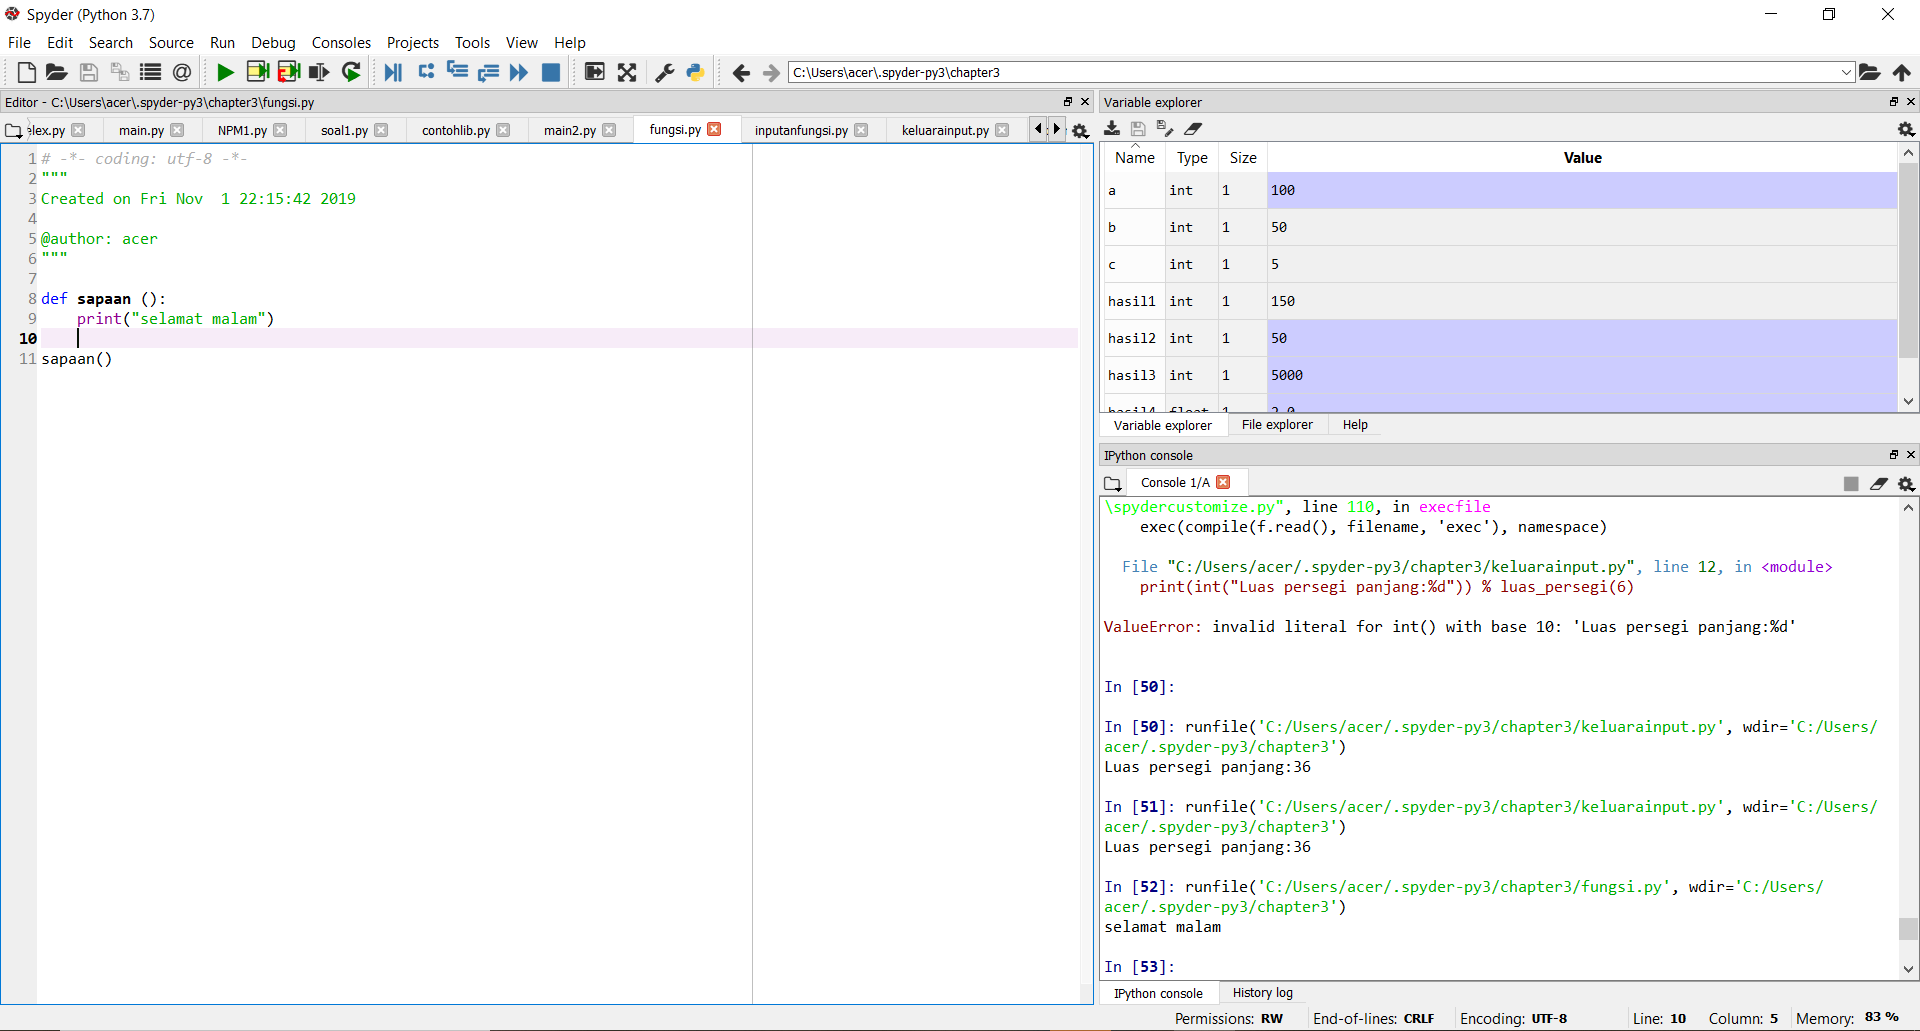
\includegraphics[width=8cm]{figures/fungsi.PNG}}
\end{figure}
\paragraph{}
    Untuk memberikan inputan pada fungsi, kita dapat menggunakan dan memanfaatkan parameter. Lalu apa itu parameter? Paremeter merupakan suatu variabel untuk menampung nilai yang akan diproses dalam fungsi.
\lstinputlisting[language=Python]{src/inputanfungsi.py}
\paragraph{}
\centerline{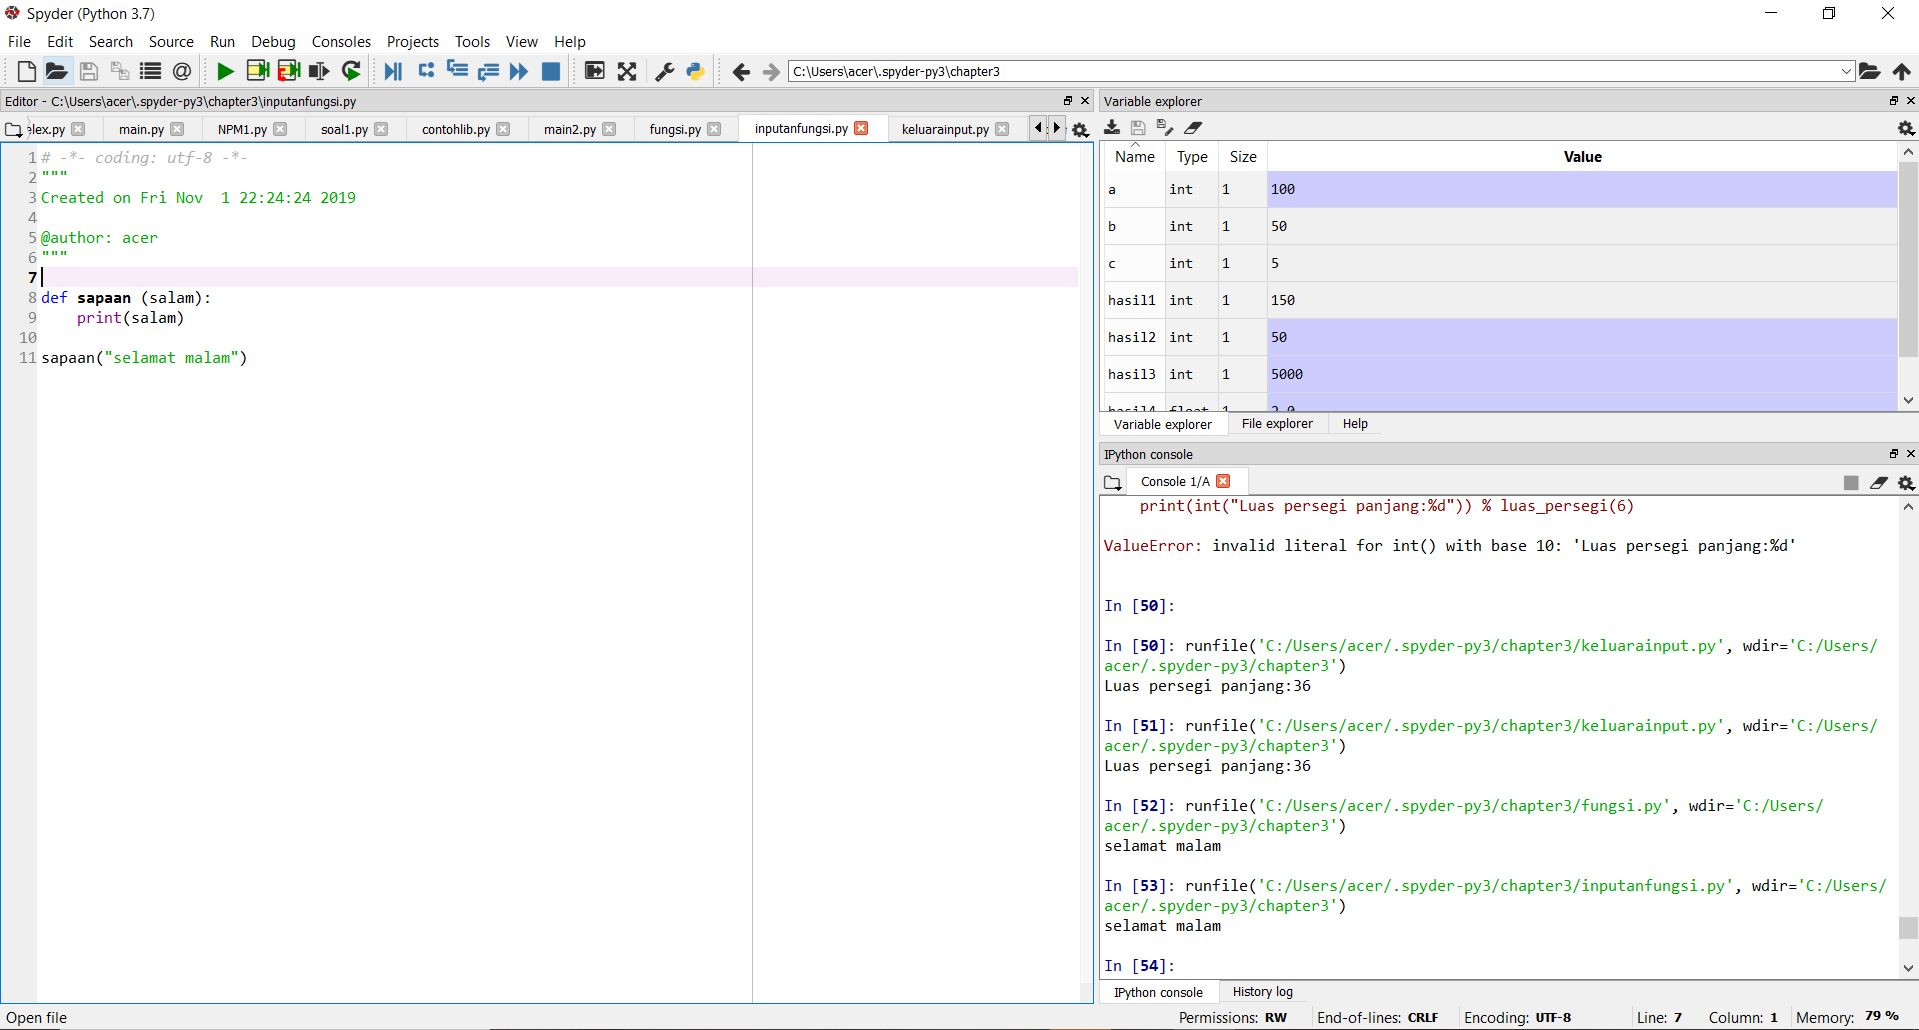
\includegraphics[width=8cm]{figures/inputanfungsi.PNG}}
\paragraph{}
    Sedangkan fungsi yang harus mengembalikan nilai bisa disebut juga keluaran fungsi, kita dapat menggunakan kata kunci \textit{return}.
\lstinputlisting[language=Python]{src/keluarainput.py}
\begin{figure}[h]
\centerline{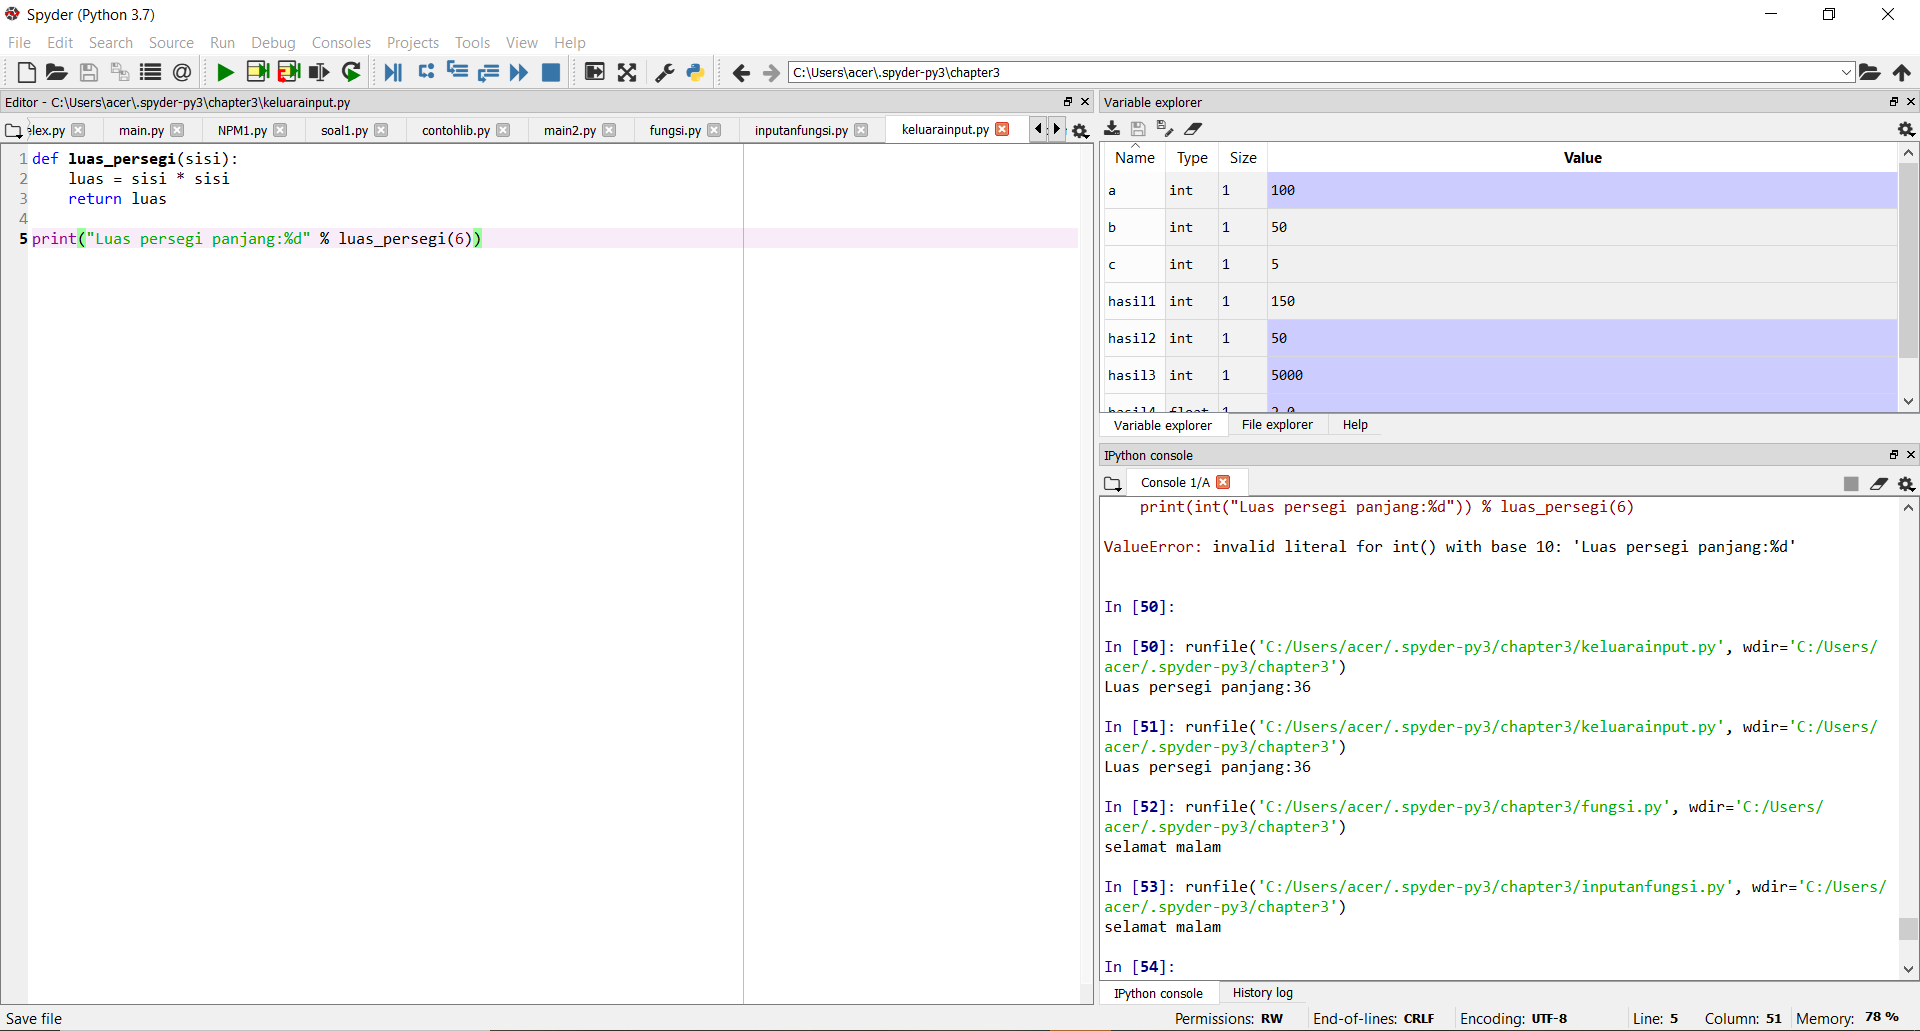
\includegraphics[width=8cm]{figures/keluaranfungsi.PNG}}
\end{figure}

\subsection{Library dan Cara Pemanggilannya}
\paragraph{}
    Library atau paket merupakan sekumpulan file-file module, sedangkan module berisikan kumpulan file dari fungsi, class, dsb. Agar suatu file dianggap paket atau package oleh python maka buatlah file \textit{init.py} terlebih dahulu.
\lstinputlisting[language=Python]{src/library.py}

\subsection{Kelas, Objek, Atribut, Method, dan Contoh Kodenya}
\paragraph{}
    Suatu prototipe yang dibuat oleh user untuk objek yang mendefinisikan atribut yang menjadi ciri objek suatu kelas. Untuk mendefinisikan suatu class, tulislah \textit{class} sebelum nama class.
\paragraph{}
    Atribut merupakan suatu data anggota sebuah variabel dan dapat diakses melalui notasi titik.
\paragraph{}
    Object Oriented Programming (OOP) adalah paradigma atau teknik pemrograman di mana semua hal dalam program dimodelkan seperti objek dalam dunia nyata. Objek merupakan suatu blueprint, di dunia nyata objek memiliki ciri atau attribut dan juga aksi atau kelakuan.
\paragraph{}
    Method merupakan suatu fungsi atau atribut yang dimiliki suatu class. Method terbagi menjadi dua jenis yaitu function dan procedure. 
\par Function merupakan bagian dari program yang memiliki algoritma tertentu dan mengembalikan suatu nilai.
\par Sedangkan Procedure mempunyai algoritma yang tidak mengembalikan nilai.
\lstinputlisting[language=Python]{src/class.py}

\subsection{Cara Memanggil Library Kelas dari Instansi dan Pemakaiannya dengan Contoh Program Lainnya}
\paragraph{}
    Berikut adalah contoh suatu file fungsi yang akan dipanggil dengan perintah \textit{form}.
\lstinputlisting[language=Python]{src/fungsi1.py}
\paragraph{}
    Berikut adalah contoh pemanggilan library.
\lstinputlisting[language=Python]{src/library1.py}

\subsection{Contoh Pemakaian Library dengan perintah from kalkulator import penambahan disertai dengan contoh kode lainnya}
\lstinputlisting[language=Python]{src/kalkulator.py}
\lstinputlisting[language=Python]{src/main.py}

\subsection{Pemanggilan paket fungsi apabila file library berada di dalam folder}
\paragraph{}
    Untuk mengakses suatu library yang berada di dalam folder, terlebih dahulu foldernya kita tulis(src) kemudian impoprt nama librarynya (library1).

\subsection{Pemakaian paket kelas apabila file library berada di dalam folder}
\paragraph{}
    Untuk mengakses suatu class dalam sebuah folder, kita perlu menuliskan nama foldernya terlebih dahulu kemudian mengimport nama kelasnya.

\newpage
\section{Ketrampilan Pemrograman}
\begin{enumerate}
\item
    \lstinputlisting[language=Python]{src/NPM1.py}
    
\item
    \lstinputlisting[language=Python]{src/NPM2.py}

\item
    \lstinputlisting[language=Python]{src/NPM3.py}
    
\item
    \lstinputlisting[language=Python]{src/NPM4.py}
    
\item
    \lstinputlisting[language=Python]{src/NPM5.py}
    
\item
    \lstinputlisting[language=Python]{src/NPM6.py}
    
\item 
    \lstinputlisting[language=Python]{src/NPM7.py}
    
\item
    \lstinputlisting[language=Python]{src/NPM8.py}

\item
    \lstinputlisting[language=Python]{src/NPM9.py}
    
\item 
    \lstinputlisting[language=Python]{src/NPM10.py}
    
\item
    \lstinputlisting[language=Python]{src/3lib.py}

\item
    \lstinputlisting[language=Python]{src/kelas3lib.py}
    \lstinputlisting[language=Python]{src/main2.py}
\end{enumerate}


\section{Ketrampilan Penanganan Error}
\begin{enumerate}
\item
\lstinputlisting[language=Python]{src/KeterampilanPenangananError.py}
\end{enumerate}

